\index{KIWI images!description|(}
\chapter{KIWI Image Description}
\label{chapter:description}
\minitoc

In order to be able to create an image with KIWI a so called
image description must be created. The image description is
represented by a directory which has to contain at least one
file named \path{config.xml} or alternatively \path{*.kiwi}.
A good start for such a description can be found in the examples
provided in \path{/usr/share/doc/packages/kiwi/examples}.

\begin{figure}[h]
\centering
\includegraphics[scale=0.5]{pictures/description.eps}
\caption{Image description directory}
\label{fig:description}
\end{figure}

The following additional information is optional for the process
of building an image but most often mandatory for the functionality
of the later operating system.

\begin{itemize}
\item \path{images.sh}\\
      Optional configuration script while creating the packed image.
      This script is called at the beginning of the image creation process.
      It is designed to clean-up the image system. Affected are all the
      programs and files only needed while the unpacked image exists.

\item \path{config.sh}\\
      Optional configuration script while creating the unpacked image. This
      script is called at the end of the installation but \emph{before}
      the package scripts have run. It is designed to configure the image
      system, such as the activation or deactivation of certain services
      (insserv). The call is not made until after the switch to the image
      has been made with \emph{chroot}.

\item \path{root/}\\
      Subdirectory that contains special files, directories, and scripts for
      adapting the image environment \textbf{after} the installation of all the
      image packages. The entire directory is copied into the root of the
      image tree using \cmd{cp -a}.

\item \path{config-yast-firstboot.xml}\\
      Configuration file for the control of the yast2 firstboot service.
      Similar to the autoyast approach yast also provides a boot time
      service called firstboot. Unfortunately there is no GUI available
      to setup the firstboot but a good documentation in
      \path{/usr/share/doc/packages/yast2-firstboot}. Once you have 
      created such a firstboot file in your image description directory, KIWI
      will process on the file and setup your image as follows:

      \begin{enumerate}
      \item KIWI enables the firstboot service.
      \item While booting the image, YaST is started in firstboot mode.
      \item The firstboot service handles the instructions listed in the
            file\linebreak \path{config-yast-firstboot.xml}.
      \item If the process finished successfully, the environment is
            cleaned and firstboot won't be called at next reboot.
      \end{enumerate}

\item \path{config-yast-autoyast.xml}\\
      Configuration file which has been created by autoyast.
      To be able to create such an autoyast profile you should first
      call:

\begin{Command}{8cm}
yast2 autoyast
\end{Command}

      Once you have saved the information from the autoyast UI as
      config-yast-autoyast.xml file in your image description directory KIWI
      will process on the file and setup your image as follows:
      \begin{enumerate}
      \item While booting the image YaST is started in autoyast mode
            automatically
      \item The autoyast description is parsed and the instructions are
            handled by YaST. In other words the \emph{system configuration}
            is performed
      \item If the process finished successfully the environment is
            cleaned and autoyast won't be called at next reboot.
      \end{enumerate}

\item \path{config-cdroot.tgz}\\
      Archive which is used for ISO images only. The data in the archive is
      uncompressed and stored in the CD/DVD root directory. This
      archive can be used, for example, to integrate a license file or
      readme information directly readable from the CD or DVD.

\item \path{config-cdroot.sh}\\
      Along with the \path{config-cdroot.tgz} one can provide a script which allows
      to manipulate the extracted data.

\item \path{config/}\\
      Optional Subdirectory that contains Bash scripts that are called
      after the installation of all the image packages, primarily in order
      to remove the parts of a package that are not needed for the operating
      system. The name of the Bash script must resemble the package name
      listed in the \path{config.xml}.
\end{itemize}

\section{The config.xml File}
The mandatory image definition file is divided into different sections
which describes information like the image name and type as well as
the packages and patterns the image should consist of.

The following information explains the basic structure of the XML document. When KIWI
is called, the XML structure is validated by a RELAX~NG based schema.
For details on attributes and values please refer to the schema
documentation file at \path{/usr/share/doc/packages/kiwi/kiwi.rng.html}.

\subsection{\xmlstarttag{image} Element}
\begin{xml}
<image schemaversion="3.5" name="iname"
 displayname="text"
 inherit="path" kiwirevision="number"
 id="10 digit number">
  <!-- ... -->
</image>
\end{xml}

The image definition starts with an \xmlstarttag{image} tag and requires the
schema format at version 2.0. The attribute \xmlattr{name} specifies the
name of the image which is also used for the filenames created
by KIWI. Because we don't want spaces in filenames the \xmlattr{name}
attribute must not have any spaces in its name.

The following optional attributes can be inserted in the \xmlstarttag{image} tag:
\begin{itemize}
\item \xmlattr{displayname}\\
      allows setup of the boot
      menu title for isolinux and grub. So you can have
      \textit{suse-SLED-foo} as the image name but something like
      \textit{my cool Image} as the boot display name.

\item \xmlattr{inherit} \\
      inherits the packages information from another image description

\item \xmlattr{kiwirevision} \\
      specifies a KIWI SVN revision number which is known to build
      a working image from this description. If the KIWI SVN
      revision is less than the specified value, the
      process will exit. The currently used SVN revision can
      be queried by calling \cmd{kiwi \option{version}}.

\item \xmlattr{id}\\
      sets an identification
      number which appears as file \path{/etc/ImageID} within the
      image.
\end{itemize}

Inside the \xmlelement{image} section the following mandatory and optional
subelements exists. The simplest image description must define the
elements \xmlstarttag{description}, \xmlstarttag{preferences}, 
\xmlstarttag{repository} and \xmlstarttag{packages} (at least one of 
\xmlattrval{type}{bootstrap}).

\subsection{\xmlstarttag{description} Element}
\begin{xml}
<description type="system">
  <author>an author</author>
  <contact>mail</contact>
  <specification>short info</specification>
</description>
\end{xml}

The mandatory \xmlelement{description} section contains information about
the creator of this image description. The attribute \xmlattr{type}
could be either of the value \xmlval{system} which indicates this is a
system image description or at value \xmlval{boot} for boot image
descriptions.

\subsection{\xmlstarttag{profiles} Element}
\begin{xml}
<profiles>
  <profile name="name" description="text"/>
  <!-- ... -->
</profiles>
\end{xml}

The optional \xmlelement{profiles} section lets you maintain one image description
while allowing for variation of the sections packages and drivers that are
included. A separate \xmlelement{profile} element must be specified for each variation.
The \xmlelement{profile} child element, which has \xmlattr{name} and \xmlattr{description} attributes,
specifies an alias name used to mark sections as belonging to a profile,
and a short description explaining what this profile does.

To mark a set of packages/drivers as belonging to a profile, simply
annotate them with the \xmlattr{profiles} attribute. It is also possible
to mark sections as belonging to multiple profiles by separating the
names in the \xmlattr{profiles} attribute with a comma.
If a packages/drivers tag does not have a profiles attribute, it is
assumed to be present for all profiles.

\subsection{\xmlstarttag{preferences} Element}
\begin{xml}
<preferences profiles="name">
  <version>1.1.2</version>
  <packagemanager>smart</packagemanager>
  <type image="name" ...>
    <ec2config|lvmvolumes|oemconfig|pxedeploy|size|split|machine>
  </type>
</preferences>
\end{xml}

The mandatory \xmlelement{preferences} section contains information about the supported
image type(s), the used packagemanager, the version of this image, and
optional attributes. The image version must be a three-part version number of
the format: \textbf{Major}.\textbf{Minor}.\textbf{Release}. In case of
changes to the image description the following rules should apply:

\begin{itemize}
\item For smaller image modifications that do not add or remove any
      new packages, only the release number is incremented.
      The \path{config.xml} file remains unchanged.
\item For image changes that involve the addition or removal of packages
      the minor number is incremented and the release number is reset.
\item For image changes that change the size of the image file
      the major number is incremented.
\end{itemize}

By default KIWI use the \cmd{smart} packagemanager but it is also possible
to use the SUSE packagemanager called \cmd{zypper}. 

In general the specification of one \xmlstarttag{preferences} section is sufficient.
However, it's possible to specify multiple \xmlstarttag{preferences} sections and
distinquish between the sections via the \xmlattr{profiles} attribute. Data
may also be shared between different profiles. Using profiles it is possible
to, for example, configure specific preferences for OEM image generation. 
Activation of a given \xmlstarttag{preferences} during image generation is triggered by
the use of the \option{add-profile} command line argument.

For each \xmlstarttag{preferences} block at least one \xmlelement{type} element must be
defined. It is possible to specify multiple \xmlstarttag{type} elements in any 
\xmlstarttag{preferences} block. To set a given \xmlstarttag{type} description as the default image
use the boolean attribute \xmlattr{primary} and set its value to \xmlval{true}.
The image type to be created is determined by the value of the \xmlattr{image}
attribute. The following list describes the supported types and possible
values of the image attribute:

\begin{itemize}
\item \xmlattrval{image}{cpio}\\
      Use the cpio image type to specify the generation os a boot image
      (intrd). When generating a boot image it is possible to specify a
      specific boot profile and boot kernel using the optional
      \xmlattrval{bootprofile}{default} and \xmlattrval{bootkernel}{std}
      attributes.
      
      A boot image should group the various supported kernels into profiles. 
      If the user chooses not to use the profiles supplied by KIWI, it is
      required that one profile named \path{std} be created. This profile
      will be used if no other bootkernel is specified. Further it is 
      required to create a  profile named \path{default}. This profile is
      used when no bootprofile is specified.

      It is recommended that special configurations that omit drivers, use
      special drivers and/or special packages be specified as profiles.


      The bootprofile and bootkernel attribute are respected within the 
      definition of a system image. Us the attribute and value 
      \xmlattrval{type}{system} of the \xmlstarttag{description} element to specify the
      creation of a system image. The values of the bootprofile and 
      bootkernel attributes are used by KIWI when generating the boot image.
\item \xmlattrval{image}{ec2}\\
      Setting the image attribute value to \xmlval{ec2} causes the generation of
      an Amazon Machine Image (AMI) for the AWS (Amazon Web Services) 
      Elastic Compute Cloud (EC2). The AMI is an image comparable to
      a VMware or Xen guest image. It can be transferred to the AWS 
      Simple Storage Service and used within the AWS infrastructure.
      Configuration of the AMI is accomplished with the optional
      \xmlelement{ec2config} element, specified as a child of the \xmlstarttag{type}
      element.

\item \xmlattrval{image}{iso}\\
      Specify the key-value pair \xmlattrval{image}{iso} to generate a live system suitable
      for deployment on optical media (CD or DVD). Use the 
      \xmlattrval{boot}{isoboot/suse-*} attribute when generating this image
      type to select the apropriate boot image for optical media. In 
      addition the optional \xmlattr{flags} attribute may be set to the
      following values with the effects described below:
      \begin{itemize}
      \item \xmlval{clic}: Creates a fuse based compressed read-only
            filesystem which allows write operations into a cow file.
      \item \xmlval{compressed}: Compressed filesystem with squashfs and
            use a link list to mount the system read-write. An additional
            split section controls the read-write information.
      \item \xmlval{unified}: Compressed filesystem with squashfs mounted
            with an aufs based overlay mount to allow read-write access.
      \end{itemize}
      %% CHECK: This sentence sounds a bit strange
      If the flags attribute is not used the filesystem will not be compressed
      and no union filesystem is used. In this case it is recommended to
      specify a \xmlelement{split} section as a child of this type element. The
      specification of a split block is also recommended when flags=compressed
      is used.
\item \xmlattrval{image}{oem}\\
      Use this type to create a virtual disk system suitable in a preload
      setting. In addition specify the attributes \xmlattr{filesystem}, 
      and \xmlattrval{boot}{oemboot/suse-*} to control the filesystem used
      for the virtual and to specify the proper boot image. Using the optional
      \xmlattr{format} attribute and setting the value to \xmlval{iso} or 
      \xmlval{usb} will create self installing images suitable for optical media
      or a USB stick, respectively. Booting from the media will deploy
      the OEM preload image onto the selected storage device of the
      system. It is also possible to configure the system to use logical
      volumes. Use the optional \xmlattr{lvm} attribute and specify the
      logical volume configuration with the \xmlelement{lvmvolumes} child
      element. The default volume group name is kiwiVG. Further configuration
      of the image is performed using the appropriate \xmlelement{*config} child
      block.
\item \xmlattrval{image}{pxe}\\
      Creating a network boot image is supported by KIWI with the 
      \xmlattrval{image}{pxe} type. When specifying the creation of a netwoork boot image use the
      \xmlattr{filesystem} and \xmlattrval{boot}{netboot/suse-*} attributes 
      to specify the filesystem of the image and the proper boot image. To
      compress the image file set the \xmlattr{compressed} boolean attribute
      to \xmlval{true}. This setting will compress the image file and has no influence
      on the filesystem used within the image. The compression is often use to
      support better transfer times when the pxe image is pushed to the 
      boot server over a network connection. The pxe image layout is
      controlled by using the \xmlelement{pxedeploy} child element.
\item \xmlattrval{image}{split}\\
      The split image support allows the creation of an image as split
      files. Using this technique one can assign different filesystems and
      different read-write properties to the different sections of the image.
      The \xmlval{oem}, \xmlattr{pxe}, \xmlattr{usb}, and \xmlattr{vmx} 
      types can be created as a split system image. Use the 
      \xmlattrval{boot}{oem|netboot\linebreak[3]|usb|vmx/suse-*} attribute
      to select the underlying type of the split image. The attributes
      \xmlattr{fsreadwrite}, \xmlattr{fsreadonly} are used to controll the
      read-write properties of the filesystem specified as the attributes
      value. Use the appropriate \xmlelement{*config} child block to specify
      the properties of the underlying image. For example when building a 
      OEM based split image use the \xmlstarttag{oemconfig} child section.
\item \xmlattrval{image}{usb}\\
      Use the usb value to create a USB stick image. Set the
      \xmlattr{filesystem} attribute to the desired supported filesystem for
      the image and use the \xmlattrval{boot}{usbboot/suse-*} attribute to
      select the USB boot image for the system. For a USB image you may
      also select GRUB or Syslinux as a bootloader by setting the
      optional \xmlattr{bootloader} attribute to grub ot syslinux,
      respectively. The USB image may also be created with LVM support.
      The same rules as indicated for the OEM image apply.
\item \xmlattrval{image}{vmx}\\
      Creation of a virtual disk system is enabled with the vmx value of
      the image attribute. Set the filesystem of the virtual disk with
      the \xmlattr{filesystem} attribute and select the appropriate boot
      image by setting \xmlattrval{boot}{vmxboot/suse-*}. The optional
      \xmlattr{format} attribute is used to specify one of the virtualization
      formats supported by qemu, such as vmdk (also the VMware format) or
      qcow2. For the virtual disk image the optional \xmlattr{vga} attribute
      may be used to configure the kernel framebuffer device. Acceptable
      values can be found in the Linux kernel documentation for the
      framebuffer device (\path{Documentation/fb/vesafb.txt}). KIWI also supports
      the selection of the booloader for the virtual disk according to
      the rules indicated for the USB system. Last but not least
      the virtual disk system may also be created with a LVM based layout by
      using the \xmlattr{lvm} attribute. The previously indicated rules apply.
      Use the \xmlelement{machine} child element
      to specify appropriate configuration of the virtual disk system.
\item \xmlattrval{image}{xen}\\
      Use this type to create a Xen para-virtual guest image. The
      \xmlattr{filesystem} and \xmlattrval{boot}{xenboot/suse-*} attributes
      specify the filesystem type used and select the proper boot image,
      respectively. Use the \xmlelement{machine} child element to specify
      configuration options of the Xen guest image.
\end{itemize}

All of the mentioned types can specify the \xmlattr{boot} attribute
which tells KIWI to call itself to build the requested boot image (initrd).
It is possible to tell KIWI to check for an already built boot image
which is a so called \emph{prebuilt boot image}. To activate searching
for an appropriate prebuilt boot image the type section also provides the
attribute \xmlattrval{checkprebuilt}{true|false}. If specified KIWI will
search for a prebuilt boot image in a directory named
\path{/usr/share/kiwi/image/*boot/*-prebuilt}. Example: If the boot
attribute was set to \xmlval{isoboot/suse-10.3} and checkprebuilt is set to true
KIWI will search the prebuilt boot image in
\path{/usr/share/kiwi/image/isoboot/suse-10.3-prebuilt}. The directory KIWI
searches for the prebuilt boot images can also be specified at the
commandline with the \option{prebuiltbootimage} parameter.

Within the preferences section there are the following optional
attributes:

\begin{itemize}
\item \xmlattr{rpm-check-signatures}\\
      Specifies whether RPM should check the package signature or not
\item \xmlattr{rpm-excludedocs}\\
      Specifies whether RPM should skip installing package documentation
\item \xmlattr{rpm-force}\\
      Specifies whether RPM should be called with \option{force}
\item \xmlattr{keytable}\\
      Specifies the name of the console keymap to use. The value corresponds
      to a map file in \path{/usr/share/kbd/keymaps}. The KEYTABLE variable in
      \path{/etc/sysconfig/keyboard} file is set according to the keyboard
      mapping.
\item \xmlattr{timezone}\\
      Specifies the time zone. Available time zones are located in the
      \path{/usr/share/zoneinfo} directory. Specify the attribute value relative to
      \path{/usr/share/zoneinfo}. For example, specify Europe/Berlin for
      \path{/usr/share/zoneinfo/Europe/Berlin}. KIWI uses this value to configure
      the timezone in \path{/etc/localtime} for the image
\item \xmlattr{locale}\\
      Specifies the name of the UTF-8 locale to use, which defines the
      contents of the RC\_LANG system environment variable in
      \path{/etc/sysconfig/language}. Please note only UTF-8 locales are supported
      here which also means that the encoding must \emph{not} be part of
      the locale information. The KIWI schema validates the locale string
      according to the following pattern:\\
      \verb+[a-z]{2}_[A-Z]{2}(,[a-z]{2}_[A-Z]{2})*+.
      This means you have to specifiy the locale like the following example:
      en\_US or en\_US,de\_DE
\item \xmlattr{boot-theme}\\
      Specifies the name of the gfxboot and bootsplash theme to use
\item \xmlattr{defaultdestination}\\
      Used if the \option{destdir} option is not specified when calling KIWI
\item \xmlattr{defaultroot}\\
      Used if the option \option{root} is not specified when calling KIWI
\item \xmlattr{defaultbaseroot}\\
      Used if the option \option{base-root} is not specified when
      calling KIWI. It's possible to prepare and create an image using a
      predefined non empty root directory as base information.
      This could speedup the build process a lot if the base root path
      already contains most of the image data.
\item \xmlattr{kernelcmdline}\\
      Specifies additional kernel parameters. The following example
      disables kernel messages: \xmlattrval{kernelcmdline}{quiet}
\end{itemize}

The \xmlstarttag{type} element may contain child elements to provide specific
configuration information for the given type. The following lists the 
supported child elements:

\begin{itemize}
\item \xmlelement{ec2config}\\
    The optional ec2config block is used to specify information relevant
    only to AWS EC2 images. The following information can be provided:

\begin{xml}
<ec2config>
  <ec2accountnr>
    Your AWS account number
  </ec2accountnr>
  <ec2certfile>
    Path to the AWS cert-*.pem file
  </ec2certfile>
  <ec2privatekeyfile>
    Path to the AWS pk-*.pem file
  </ec2privatekeyfile>
</ec2config>
\end{xml}

\item \xmlelement{lvmvolumes}\\
	Using the optional \xmlelement{lvmvolumes} section it possible to create
    a LVM (Logical Volume Management) based storage layout. By default the
    volume group is named kiwiVG. It is possible to change the name of the
    group by setting the \xmlattr{lvmgroup} attribute to the desired name.
    Individual volumes within the volume group are specified using the 
    \xmlelement{volume} element. 

    The following example shows the creation of a volume named usr and a
    volume named var inside the volume group systemVG.

\begin{xml}
<lvmvolumes lvmgroup="systemVG">
  <volume name="usr" freespace="100M"/>
  <volume name="var" size="200M"/>
</lvmvolumes>
\end{xml}

	With the optional \xmlattr{freespace} attribute it is possible to
    add space to the volume. If the freespace attribute is not set the
    created volume will be 80\,\% to 90\,\% full. Using the optional
    \xmlattr{size} attribute the absolute size of the given volume is
    specified. The size attribute takes precedence over the freespace
    attribute. Should the specified size be too small the value will
    be ignored and a volume with approximately 80\,\% to 90\,\% fill will
    be created.

\item \xmlelement{oemconfig}
	By default the oemboot process will create/modify a swap, \path{/home} and 
	\path{/} partition. It is possible to influence the behavior by the
	\xmlelement{oem-*} elements explained below.
	KIWI uses this information to create the file
	\path{/config.oempartition} as part
	of the automatically created oemboot boot image. The format of the
	file is a simple key=value format and created by the \cmd{KIWIConfig.sh}
	function named baseSetupOEMPartition(). 

\begin{xml}
<oemconfig>
  <oem-systemsize>2000</oem-systemsize>
  <oem-... >
</oemconfig>
\end{xml}

	\begin{itemize}
    \item \xmlstarttag{oem-boot-title}text\xmlendtag{oem-boot-title}\\
       By default the string \verb!OEM! will be used as the boot manager 
       menu entry when KIWI creates the grub configuration during
       deployment. The oem-boot-title element allows you to set a custom
       name for the grub menu entry. This value is represented by the
       OEM\_BOOT\_TITLE variable in \path{config.oempartition}.
	\item \xmlstarttag{oem-home}true|false\xmlendtag{oem-home>}\\
       Specify if a partition for the home directory should be created.
       Creation of a home partition is the default behavior. This value is 
       represented by the OEM\_WITHOUTHOME variable in config.oempartition.
	\item \xmlstarttag{oem-kiwi-initrd}true|false\xmlendtag{oem-kiwi-initrd}\\
       If this element is set to true (default value is false) the oemboot 
       boot image (initrd) will \emph{not} be replaced by the system 
       (mkinitrd) created initrd. This option is useful when the system
       is installed on removable storage such as a USB stick or a portable
       external drive. For movable devices it is potentially necessary to 
       detect the storage location during every boot. This detection
       process is part of the oemboot boot image. This value is represented
       by the OEM\_KIWI\_INITRD variable in \path{config.oempartition}.
	\item \xmlstarttag{oem-reboot}true|false\xmlendtag{oem-reboot}\\
       Specify if the system is to be rebooted after the oem image has been
       deployed to the designated storage device (default value is false). 
       This value is represented by the OEM\_REBOOT variable in 
       \path{config.oempartition}.
	\item \xmlstarttag{oem-recovery}true|false\xmlendtag{oem-recovery}\\
      If this element is set to true (default value is \xmlval{false}), KIWI will
      create a recovery archivefrom the prepared root tree. The archive will 
      appear as \path{/recovery.tar.bz2} in the image file. During 
      first boot of the image a single recovery partition will be
      created and the recovery archive will be moved to the recovery 
      partition. An additional boot menu entry is created that when selected
      restores the original root tree on the system. The
      user information on the \path{/home} partition or in the \path{/home} directory is
      not affected by the recovery process. This value is represented by 
      the OEM\_RECOVERY variable in \path{config.oempartition}.
    \item \xmlstarttag{oem-recoveryID}partition-id\xmlendtag{oem-recoveryID}\\
      Specify the partition type for the recovery partition. The default 
      is to create a Linux partition (id\,=\,83). This value is represented by 
      the OEM\_RECOVERY\_ID variable in config.oempartition. 
    \item \xmlstarttag{oem-swap}true|false\xmlendtag{oem-swap}\\
       Specify if a sawp partition should be create. The creation of a swap
       partition is the default behavior. This value is represented by the
       OEM\_WITHOUTSWAP variable in config.oempartition.
    \item \xmlstarttag{oem-swapsize}number in MB\xmlendtag{oem-swapsize}\\
       Set the size of the swap partition. If a swpa partition is to be
       created and the size of the swap partition is not specified with this
       optional element, KIWI will calculate the size of the swpar partition
       and create a swap partition equal to two times the RAM installed on
       the system at initial boot time. This value is represented by
       the OEM\_SWAPSIZE variable in config.oempartition
    \item \xmlstarttag{oem-systemsize}number in MB\xmlendtag{oem-systemsize}\\
      Set the size of the root partition. This value is represented by the
      variable OEM\_SYSTEMSIZE in config.oempartition
	\end{itemize}

\item \xmlelement{pxedeploy}\\
    Information contained in the optional pxedeploy section is only considered
    if the \xmlattr{image} attribute of the \xmlelement{type} element is set to
    \xmlval{pxe}. In order to use a PXE image it is necessary to create a
    network boot infrastructure. Creation of the network boot infrastructure
    is simplified by the KIWI provided package kiwi-pxeboot. This
    package configures the basic PXE boot enviroment as expected by KIWI pxe
    images. The kiwi-pxeboot package creates a directory structure in
    \path{/srv/tftpboot}. Files created by the KIWI create step need to be copied
    to the \path{/srv/tftpboot} directory structure. For additional details about
    the PXE image please refere to the PXE Image chapter later in this
    document.

    In addition to the image files it is necessary that information be
    provided about the client setup. This information, such as the image
    to be used or the partitioning, is contained in a file with the name
    \path{config.<MAC-Address>} in the directory \path{/srv/tftpboot/KIWI}. The content
    of this file is created automatically by KIWI if the pexedeploy section
    is provided in the image description. A pxedeploy section is outlined
    below:

\begin{xml}
<pxedeploy server="IP" blocksize="4096">
  <timeout>seconds</timeout>
  <kernel>kernel-file</kernel>
  <initrd>initrd-file</initrd>
  <partitions device="/dev/sda">
    <partition type="swap" number="1" size="MB"/>
    <partition type="L" number="2" size="MB"
      mountpoint="/" target="true"/>
    <partition type="fd" number="3"/>
  </partitions>
  <union ro="dev" rw="dev" type="aufs|clicfs|unionfs"/>
  <configuration source="/KIWI/../file" dest="/../file"
                 arch="..."/>
  <configuration .../>
</pxedeploy>
\end{xml}

	\begin {itemize}
	\item The \xmlattr{server} attribute is used to specify the IP address
      of the PXE server. The \xmlattr{blocksize} attributes specifies the
      blocksize for the image download. Other protocols are supported by
      KIWI but require the \xmlval{kiwiserver} and \xmlval{kiwiservertype}
      kernel parameters to be set when the client boots.
	\item The value of the optional timeout element specifies the grub
      timeout in seconds to be used when the KIWI initrd configures and
      installs the grub boot loader on the client machine after the first
      deployment to allow standalone boot.
	\item Passing kernel parameters is possible with the use of the
      optional kernelcmdline attribute in the \xmlstarttag{type} section. The value
      of this attribute is a string specifying the settings to be
      passed to the kernel by the grub bootloader. The KIWI initrd
      includes these kernel options when installing grub for standalone boot
	\item The optional \xmlelement{kernel} and \xmlelement{initrd} elements are
      used to specify the file names for the kernel and initrd on the boot
      server respectively. When using a special boot method not supported
      by the distribution's standard mkinitrd, it is imperative that the
      KIWI initrd remains on the PXE server and also be used for local boot.
      If the configured image uses the \xmlelement{split} type or the \xmlelement{pexedeploy}
      section includes any union information the kernel and initrd elements
      must be used.
	\item The \xmlelement{partitions} section is required if the system image is to be
      installed on a disk or other permanent storage device. Each partition
      is specified with one partition child element. The mandatory
      \xmlattr{type} attribute specifies the partition type. The possible
      values are the sfdisk supported types, use the following command
      to obtain a list of supported values:
      
\begin{Command}{14cm}
sfdisk --list-type
\end{Command}
      
      The required \xmlattr{number}
      attribute provides the the number of the partition to be created. The
      size of the partition may be specified with the optional \xmlattr{size}
      attribute. The optional \xmlattr{mountpoint} attribute provides
      the value for the mount point of the partition. The optional boolean
      \xmlattr{target} attribute identifies the partion as the system image
      target partition.
      KIWI always generates the swap partition as the first partition of
      the netboot boot image. By default the second partition is used for
      the system image. Use the boolean target attribute to change this
      behavior. Providing the value \xmlval{image} for the \xmlattr{size} attribute
      triggers KIWI into calculating the required size for this partition.
      The calculated size is sufficient for the created image.
	\item If the system image is based on a read-only filesystem such as
      squashfs and should be mounted in read-write mode use the optional
      \xmlelement{union} element. The \xmlattr{type} attribute is used to specify
      one of the supported overlay filesystem (aufs, clicfs, or unionfs).
      Use the \xmlattr{ro} attribute to point to the read only device and
      the \xmlattr{rw} attribute to point to the read-write device.
	\item The optional configuration element is used to integrate a network
      client's configuration files that are stored on the server.
      The \xmlattr{source} attribute specifies the path on the server for
      the file to be downloaded. The \xmlattr{dest} attribute specifies
      destination of the downloaded file on the network client starting at
      the root (\path{/}) of the filesystem. Multiple configuration elements
      may be specified such that multiple files can be transferred to the
      network client. In addition configuration files can be bound to
      a specific client architecture by setting the optional \xmlattr{arch}
      attribute. To specify multiple architectures use a comma separated
      string.
	\end{itemize}

\item \xmlelement{size}\\
    Use the size element to specify the image size in Megabytes or
    Gigabytes. The \xmlattr{unit} attribute specifies whether the given
    value will be interpreted as Megabytes (\xmlattrval{unit}{M}) or
    Gigabytes (\xmlattrval{unit}{G}). The optional boolean attribute
    \xmlattr{additive} specifies whether or not the given size should be added
    to the size of the generated image or not.

    In the event of a size specification that is too small for the
    generated image, KIWI will expand the size automatically unless the
    image size exceeds the specified size by 100\,MB or more. In this case
    KIWI will generate an error and exit.

    Should the given size exceed the necessary size for the image KIWI will
    not alter the image size as the free space might be required for proper
    execution of components within the image.

    If the size element is not used KIWI will create an image with
    containing approxiamtely 30\,\% free space.
    
     
\begin{xml}
<size unit="M">1000</size>
\end{xml}

\item \xmlelement{split}\\
    For images of type split or iso the information provided in the optional
    split section is is considered if the \xmlattr{compressed} attribute is
    is set to \xmlval{true}. With the configuration in this block it is
    possible to determine which files are writable and whether these files
    should be persentently writable or temporarily. Note that for ISO images
    only temporary write access is possible.

    When processing the provided configuration KIWI distinguishes between
    directories and files. For example, providing \path{/etc} as the value of
    the \xmlval{name} attribute indicates that the \path{/etc} directory should be
    writable. However, this does not include any of the files or 
    sub-directories within \path{/etc}. The content of \path{/etc} is populated as 
    symbolic links to the read-only files. The advantage of setting only a
    directory to read-write access is that any newly created files will be
    stored on the disk instead of in tmpfs. Creating read-write access to a 
    directory and it's files requires two specifications as showb below.

\begin{xml}
<split>
  <temporary>
    <!-- read/write access to: -->
    <file name="/var"/>
    <file name="/var/*"/>
    <!-- but not on this file: -->
    <except name="/etc/shadow"/>
  </temporary>
  <persistent>
    <!-- persistent read/write access to: -->
    <file name="/etc"/>
    <file name="/etc/*"/>
    <!-- but not on this file: -->
    <except name="/etc/passwd"/>
  </persistent>
</split>
\end{xml}

    Use the \xmlelement{except} element to specify exceptions to previously
    configured rules.

\item \xmlelement{machine}\\
    The optional machine section serves to specify information
    about a VM guest machine. Using the data provided in this section,
    KIWI will create a guest configuration file required to run the
    image on the target machine.

    If the target is a VMware virtual machine indicated by the
    format attribute set to vmdk, KIWI creates a VMware configuration file.
    If the target is a Xen virtual machine indicated by the domain
    attribute in the machine section KIWI will create a Xen guest
    config file.

    The sample block below shows the general outline of the information
    that can be specified to generate the configuration file

\begin{xml}
<machine arch="arch" memory="MB" HWversion="number"
         guestOS="suse|sles" domain="dom0|domU"/>
  <vmnic driver="name" interface="number" mode="mode"/>
  <vmdisk controller="ide|scsi" id="number"/>
  <vmdvd controller="ide|scsi" id="number"/>
</machine>
\end{xml}

	\begin{itemize}
	\item \xmlattr{arch}\\
      The virtualized architecture. Supported values are ix86 or x86\_64.
      The default value is \xmlval{ix86}.
	\item \xmlattr{memory}\\
      The mandatory \xmlattr{memory} attribute specifies how much memory in MB
      should be allocated for the virtual machine
	\item \xmlattr{HWversion}\\
      The VMware hardware version number, the default value is 3.
	\item \xmlattr{guestOS}\\
      The guestOS identifier. For the ix86 architecture the default 
      value is \xmlval{suse} and for the x86\_64 architecture
      \xmlval{suse-64} is the default. At this point only the SUSE and
      SLES guestOS types are supported.
	\item \xmlattr{domain}\\
      The Xen domain setup. This could be either a dom0 which is the
      host machine hosting the guests and therefore doesn't require a
      configuration file, or it could be set to domU which indicates
      this is a guest and also requires a guest configuration which is
      created by KIWI.
	\end{itemize}

	The following information can be provided to setup the virtual
	main storage device and CD/DVD drive connection:

	\begin{itemize}
	\item \xmlattr{controller}\\
      Supported values for the mandatory controller attribute are \xmlval{ide}
      and \xmlval{scsi}.
	\item \xmlattr{id}\\
      The mandatory \xmlattr{id} attribute specifies the disk id. If only one
      disk is set the id value should be set to 0.
	\item \xmlattr{device}\\
      The device attribute specifies the disk that should appear
      in the para virtual instance. Therefore only relevant for Xen
	\end{itemize}

	The following information can be provided to setup the virtual
	network interface:

	\begin{itemize}
	\item \xmlattr{driver}\\
      The mandatory \xmlattr{driver} attribute specifies the driver to be used for
      the virtual network card. The supported values are \xmlval{e100},
      \xmlval{vlance}, and \xmlval{vmxnet}. If the vmxnet driver is
      specified the \xmlval{vmware tools} must be installed in the image.
	\item \xmlattr{interface}\\
      The mandatory \xmlattr{interface} attribute specifies the interface number. If
      only one interface is set the value should be set to 0.
	\item \xmlattr{mode}\\
      The network mode used to communicate outside the VM. In many cases
      the bridged mode is used.
	\end{itemize}
\end{itemize}

\subsection{\xmlstarttag{users} Element}
\begin{xml}
<users group="group_name" id="number">
  <user home="dir" id="number" name="user" pwd="..."
        pwdformat="encrypted|plain"
        realname="string" shell="path/>
  <!-- ... -->
</users>
\end{xml}

The optional \xmlelement{users} element lists the users belonging to the group specified
with the \xmlattr{group} attribute. At least one user child element must be specified
as part of the \xmlelement{users} element. Multiple users elements may be specified.

The attributes \xmlattr{home}, \xmlattr{id}, \xmlattr{name}, \xmlattr{pwd}, 
\xmlattr{realname}, and \xmlattr{shell} specify the created
users home directory, the user name, the user's password, the user's 
real name, and the user's login shell, respectively. By default the value
of the password attribute is expected to be an encrypted string. An
encrypted password can be created using \cmd{kiwi \option{createpassword}}. It
is also possible to specify the password as a non encrypted string by using
the \xmlattr{pwdformat} attribute and setting it's value to \kquote{plain}. KIWI will then
encrypt the password prior to the user being added to the system.

All specified users and groups will be created if they do not already exist.
By default the defined users will be part of the group specified with the 
group attribute of the users element and the default group called \kquote{users}.
If it is desired to have the specified users to only be part of the given
group it is necessary to specify the id attribute. It is recommended to use
a group id greater than 100.

\subsection{\xmlstarttag{drivers} Element}
\begin{xml}
<drivers type="type" profiles="name">
  <file name="filename"/>
  <!-- ... -->
</drivers>
\end{xml}

The optional \xmlelement{drivers} element is only useful for boot images (initrd).
As a boot image doesn't need to contain the complete kernel one can
save a lot of space if only the required drivers are part of the image.
Therefore the drivers section exists. If present only the drivers which
matches the file names or glob patterns will be included into the
boot image. The \xmlattr{type} attribute specifies one of the following driver
types:

\begin{itemize}
\item \xmlelement{drivers}\\
      Each file is specified relative to the
      \path{/lib/modules/<Version>/kernel} directory.
\item \xmlelement{netdrivers}\\
      Each file is specified relative to the
      \path{/lib/modules/<Version>/kernel/drivers}
      directory.
\item \xmlelement{scsidrivers}\\
      Each file is specified relative to the
      \path{/lib/modules/<Version>/kernel/drivers}
\item \xmlelement{usbdrivers}\\
      Each file is specified relative to the
      \path{/lib/modules/<Version>/kernel/drivers} directory.
\end{itemize}

According to the driver type the specified files are searched in
the corresponding directory. The information about the drivernames
is provided as environment variable named like the value of
the type attribute and is processed by the function
\texttt{suseStripKernel}. According to this along with a boot image
description a script called \cmd{images.sh} must exist which
calls this function in order to allow the driver information to
have any effect.

%\newpage

\subsection{\xmlstarttag{repository} Element}
\begin{xml}
<repository type="type" status="replaceable"
            alias="name" priority="number">
  <source path="URL"/>
</repository>
\end{xml}

The mandatory \xmlelement{repository} element specifies the source URL and
type used by the package manager. The type attribute specifies the
repository type which must be supported by the package manager.
At the moment KIWI supports the package managers smart and zypper
whereas smart has support for more repository types compared to
zypper. Therefore the possible values for the type attribute has
beend copied from smart. The following table shows the possible
repo types:\\ 

\begin{longtable}[h]{|p{4cm}|p{3cm}|p{3cm}|}
\hline
\textbf{Type} & \textbf{smart Support} & \textbf{zypper Support}\\
\hline 
apt-deb            & yes & no  \\
apt-rpm            & yes & no  \\
deb-dir            & yes & no  \\
mirrors            & yes & no  \\
red-carpet         & yes & yes \\
rpm-dir            & yes & yes \\
rpm-md             & yes & yes \\ 
slack-site         & yes & no  \\
up2date-mirrors    & yes & no  \\
urpmi              & yes & no  \\
yast2              & yes & yes \\
\hline
\end{longtable}

Within the repository section there are the following optional
attributes:

\begin{itemize}
\item \xmlattrval{status}{replaceable}\\
      This attribute makes only sense for boot image descriptions.
      It indicates that the repository is allowed to become replaced by
      the repositories defined in the system image descriptions. Because KIWI
      automatically builds the boot image if required it should create that
      image from the same repositories which are used to build the system
      image to make sure both fit together. Therefore it is required to allow
      the repository to become overwritten which is indicated by the status
      attribute.
\item \xmlattrval{alias}{name}\\
      Specifies an alternative name used to identify the source channel.
      If not set the source attribute value is used and builds the alias name
      by replacing each \kquote{/} with a \kquote{\_}. An alias name should be set if
      the source argument doesn't really explain what this repository
      contains 
\item \xmlattrval{priority}{number}\\
      Specifies the repository priority assigned to all packages available in
      this repository. For \cmd{smart} the following applies: If the
      exact same package is available in more than one channel, the repository
      with the \emph{highest} priority number is used. The value 0 means
      \kquote{no priority is set}. For \cmd{zypper} the following applies:
      If the exact same package is available in more than one channel, the
      repository with the \emph{lowest} priority number is used. The value
      99 means \kquote{no priority is set}.
\end{itemize}

The source child element contains the path attribute, which specifies
the location (URL) of the repository. The path specification can be any
of the following, and can include the \%arch macro which is expanded
to the architecture of the image building host.

\begin{itemize}
\item \path{this://<path>}\\
      A relative path name, which is relative to the image
      description directory being referenced.
\item \path{iso://<path/to/isofile>}\\
      A path to a local \path{.iso} file which is then loopback mounted
      and used as a local path based repository. Alternatively one
      can do the loop mount himself and point a standard local path
      to the mounted directory
\item \path{http://<url>}\\
      A http protocol based network location
\item \path{https://<url>}\\
      A https protocol based network location
\item \path{ftp://<url>}\\
      A ftp protocol based network location
\item \path{opensuse://<Project-Name>}\\
      A special http based network location which is created from
      the given openSUSE buildservice project name. The result is
      pointing to an rpm-md repository on the openSUSE buildservice.
      For example: %\\
      \xmlattrval{path}{\path{opensuse://openSUSE:10.3/standard}}
\item \path{file:///local/path}\\
      A local path which should be an absolute path description.
      The \path{file://} prefix is optional and could also be omitted.
\item \path{obs://$dir1/$dir2}\\
      A special buildservice path whereas \path{$dir1} and \path{$dir2}
      represents the buildservice project location. If this type is
      used as part of a boot attribute KIWI evaluates it to
      \path{this://images/$dir1/$dir2} and if used as part of a repository
      source path attribute it evaluates to \path{this://repos/$dir1/$dir2}
\end{itemize}

Multiple repository sections are allowed and combined by the
used package manager. By default the package manager will always use
the latest packages available.

\subsection{\xmlstarttag{packages} Element}
\begin{xml}
<packages type="type" profiles="name" patternType="type" patternPackageType="type"
  <package name="name" arch="arch"/>
  <package name="name" replaces="name"/>
  <package name="name" bootinclude="true" bootdelete="true"/>
  <archive name="name" bootinclude="true"/>
  <package .../>
  <opensusePattern name="name"/>
  <opensusePattern .../>
  <opensuseProduct name="name"/>
  <opensuseProduct .../>
  <ignore name="name"/>
  <ignore .../>
</packages>
\end{xml}

The mandatory \xmlelement{packages} element specifies the list of packages 
(element \xmlstarttag{package}) and patterns (element \xmlstarttag{opensusePattern}) 
to be used with the image.
The value of the type attribute specifies how the packages and patterns 
listed are handled, supported values are as follows:

\begin{itemize}
\item \xmlval{bootstrap}\\
      Bootstrap packages, list of packages for the new operating system
      root tree. The packages list the required components to support a 
      chroot environment in the new system root tree, such a glibc.
\item \xmlval{delete}\\
      Delete packages, list of packages to be deleted from the image being
      created.

      When using the delete type only \xmlstarttag{package} elements are considered, all
      other specifications such as \xmlstarttag{opensusePattern} are ignored. The given
      package names are stored in the \$delete environment variable of the 
      \path{/.profile} file created by KIWI. The list of package names is returned 
      by the baseGetPackagesForDeletion() function. This list can then be
      used to delete the packages ignoring requirements or dependencies. 
      This can be accomplished in the \cmd{config.sh} or \cmd{images.sh} script with
      the following code snippet:
\begin{Command}
rpm -e --nodeps --noscripts \
  $(rpm -q `baseGetPackagesForDeletion` | grep -v "is not installed")
\end{Command}

      Note, that the delete value is indiscriminate of the image type
      being built.
\item \xmlval{image}\\
      Image packages, list of packages to be installed in the image.
\item \xmlval{iso}\\
      Image packages, a list of additional packages to be installed 
      when building an ISO image.
\item \xmlval{oem}\\
      Image packages, a list of additional packages to be installed 
      when building an OEM image.
\item \xmlval{pxe}\\
      Image packages, a list of additional packages to be installed 
      when building an PXE image.
\item \xmlval{usb}\\
      Image packages, a list of additional packages to be installed 
      when building a USB image.
\item \xmlval{vmx}\\
      Image packages, a list of additional packages to be installed 
      when building a vmx virtual image of any format.
\item \xmlval{xen}\\
      Image packages, a list of additional packages to be installed 
      when building a Xen host or guest.
\end{itemize}

\subsubsection{Using Patterns}
Using a pattern name enhances the package list with a number of
additional packages belonging to this pattern. Support for patterns
is SUSE-specific, and available with open\-SUSE 10.1 or later.
The optional patternType and patternPackageType attributes specify
which pattern references or packages should be used in a given pattern.
The values of these attributes are only evaluated, if the KIWI pattern
solver is used. If the new (up to SUSE~11.0) satsolver pattern solver
is used these values are ignored because the satsolver can't handle
that at the moment. Allowed values for the \xmlattr{pattern*} attributes are:

\begin{itemize}
\item \xmlval{onlyRequired}\\
      Incorporates only patterns and packages that are required by the
      given pattern
\item \xmlval{plusSuggested}\\
      Incorporates patterns and packages that are required
      and suggested by the given pattern
\item \xmlval{plusRecommended}\\
      Incorporates patterns and packages that are required and
      recommended by the given pattern.
\end{itemize}

By default, only required patterns and packages are used. The result
list of packages is solved into a clean conflict free list of packages
by the package manager. This for example means that including a suggested
package may include required and recommended packages as well according
to the dependencies. If a pattern contains unwanted packages, you can use
the ignore element to specify an ignore list, with the name attribute
containing the package name. Please note that you can't ignore a package
if it is required by a package dependency of another package in your list.
The packagemanager will automatically pull in the package even if you have
ignored it.

\subsubsection{Architecture Restrictions}
To restrict a package to a specific architecture, use
the \xmlattr{arch} attribute to specify a comma separated list of allowed
architectures. Such a package is only installed if the build systems
architecture (\cmd{uname -m}) matches one of the specified values of the arch
attribute.

\subsubsection{Image Type Specific Packages}
If a package is only required for a specific type of image
and replaces another package you can use the \xmlattr{replaces} attribute
to tell KIWI to install the package by replacing another one. For example
you can specify the kernel package in the \xmlattrval{type}{image} section as

\begin{xml}
<package name="kernel-default" replaces="kernel-xen"/>
\end{xml}

and in the \xmlattrval{type}{xen} section as

\begin{xml}
<package name="kernel-xen" replaces="kernel-default"/>
\end{xml}

The result is the xen kernel if you request a xen image and the
default kernel in any other case.

\subsubsection{Packages to Become Included Into the Boot Image}
The optional attributes \xmlattr{bootinclude} and \xmlattr{bootdelete}
can be used to mark a package inside the system image description to
become part of the corresponding boot image (initrd). This feature
is most often used to specify bootsplash and/or graphics boot related
packages inside the system image description but they are required
to be part of the boot image as the data is used at boot time
of the image. If the bootdelete attribute is specified along with
the bootinclude attribute this means that the selected package
will be marked as a \kquote{to become deleted} package and is
removed by the contents of the \cmd{images.sh} script of the corresponding
boot image description

\subsubsection{Data not Available as Packages to Become Included}
With the optional \xmlelement{archive} element it's possible to include
any kind of data into the image. The archive elements expects the
name of a tarball which must exist as part of the system image
description. KIWI then picks up the tarball and installs it into
the image. If the \xmlattr{bootinclude} attribute is set along with
the archive element the data will also become installed into the
boot image.



